\begin{frame}{SRCNN}
    \begin{block}{Imagenes baja resolución}
        Para obtener las imagenes en baja resolución:
        \begin{enumerate}
            \item 91 imagenes, tomadas de \textbf{ImageNET}, \textbf{Set14} y \textbf{set5}.
            \item Reescalar imagen a un factor $\frac{1}{n}$
            \item Reescalar imagen a un factor $n$
        \end{enumerate}
    \end{block}
    Desarrollo de modelos para factores de escalamiento $4$ y $2$.
    \begin{figure}[H]
        \label{fig:SRCNN_BajaAltaRes}
        \centering
        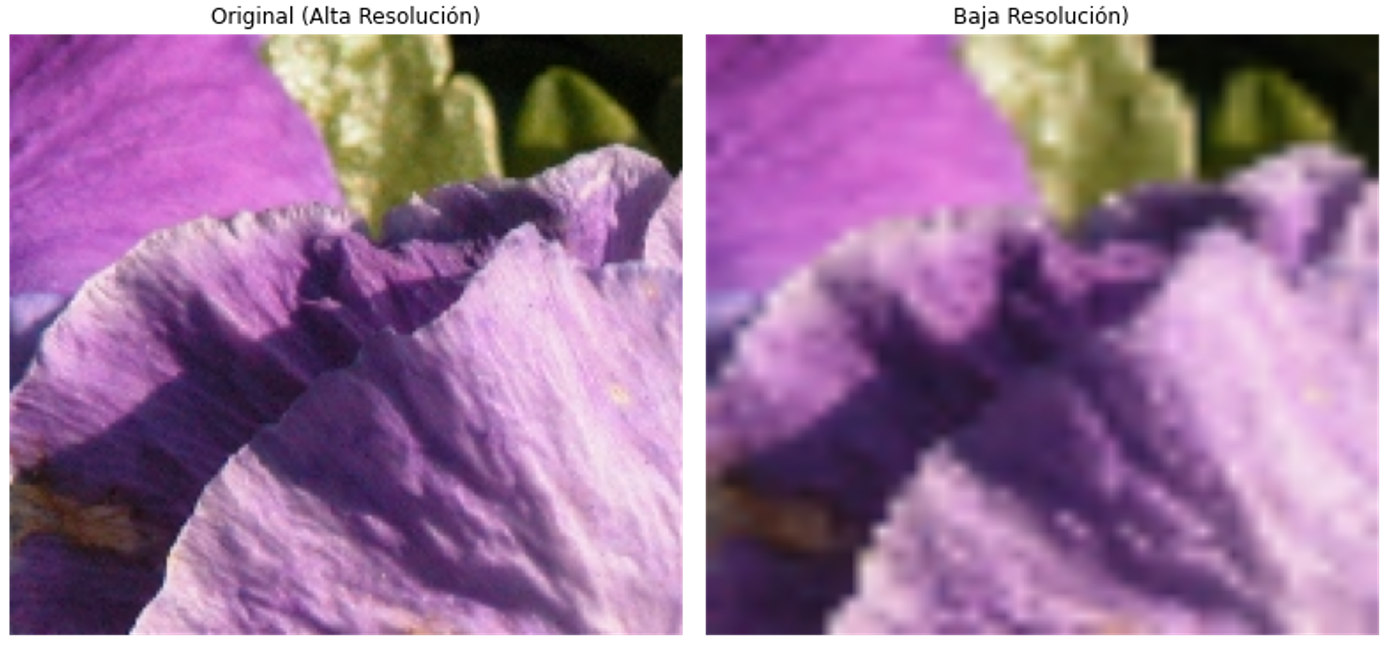
\includegraphics[scale = 0.2]{SRCNN_BajaAlta_Res.png}
        \caption{Imagen baja resolución factor de escalamiento $4$}
    \end{figure}
\end{frame}

\begin{frame}{Paramétros de modelo SRCNN}
    Los diseños de la red neuronal convolucional tienen la siguiente estructura:
    \begin{table}[H]
        \centering
        \caption{Red convolucional para espacio de color $YC_rC_b$}
        \resizebox{10cm}{!}{
        \begin{tabular}{|l|l|l|l|l|}
        \hline
        \textbf{Capa} & \textbf{Filtros} & \textbf{Kernel}  & \textbf{Inicializador de Kernel} & \textbf{Función de activación}\\ \hline
        1             & 128              & $9\times9$       & \emph{Glorot\_Uniform}           & ReLU                 \\
        2             & 64               & $5\times5$       & \emph{Glorot\_Uniform}           & ReLU                 \\
        3             & 1                & $5\times5$       & \emph{Glorot\_Uniform}           & Lineal               \\ \hline
        \end{tabular}
        }
    \end{table}

    \begin{table}[H]
        \centering
        \caption{Red convolucional para espacio de color $RGB$}
        \resizebox{10cm}{!}{
        \begin{tabular}{|l|l|l|l|l|}
        \hline
        \textbf{Capa} & \textbf{Filtros} & \textbf{Kernel}  & \textbf{Inicializador de Kernel} & \textbf{Función de activación}\\ \hline
        1             & 128              & $9\times9$       & \emph{Glorot\_Uniform}           & ReLU                 \\
        2             & 64               & $5\times5$       & \emph{Glorot\_Uniform}           & ReLU                 \\
        3             & 3                & $5\times5$       & \emph{Glorot\_Uniform}           & Lineal               \\ \hline
        \end{tabular}
        }
    \end{table}
\end{frame}

\begin{frame}{Diseño de optimizador de entrenamiento SRCNN}
    \begin{table}[H]
        \centering
        \caption{Parámetros de entrenamiento del optimizador \textbf{Adam}}
        \resizebox{10cm}{!}{
        \begin{tabular}{|l|l|l|l|l|l|}
        \hline
        \textbf{Capa} & \textbf{$\beta_1$} & \textbf{$\beta_2$}  & \textbf{$\alpha$ menor a 150 epocas} & \textbf{$\alpha$ mayor o igual a 150 epocas} & \textbf{$\epsilon$}\\ \hline
        1             & 0.9           & 0.999          & 0.003                                        & 0.001                                        & 1e-9                 \\
        2             & 0.9           & 0.999          & 0.003                                        & 0.001                                        & 1e-9                 \\
        3             & 0.9           & 0.999          & 0.0003                                       & 0.0001                                       & 1e-9                 \\ \hline
        \end{tabular}
        }
    \end{table}
\end{frame}

\begin{frame}{Proceso de entrenamiento modelo $RGB$ y factor $4$}
    \begin{figure}[H]
        \centering
        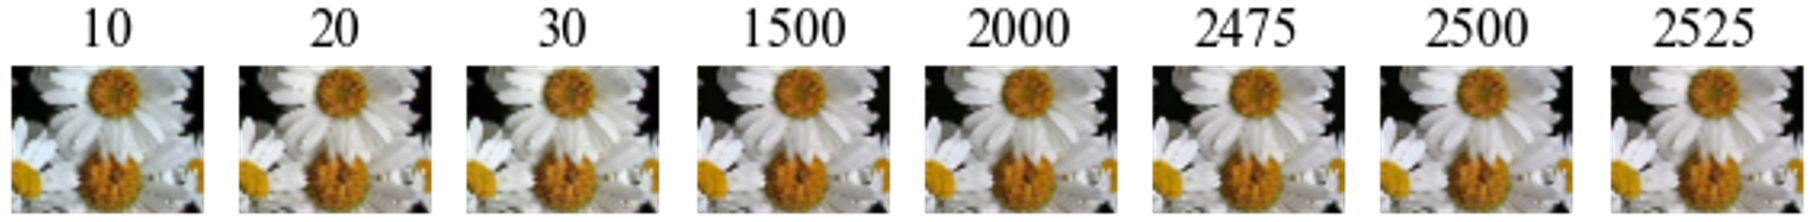
\includegraphics[width=10cm, height=1cm]{ProcesoEntrenamiento_RGB4.png}
        \caption{Proceso de aprendizaje de la red convolucional $RGB$ con factor de escalamiento de $4$}
        \label{fig:SRCNN_MSE_TrainingProcess4RGB}
    \end{figure}
    \begin{figure}[H]
        \centering
        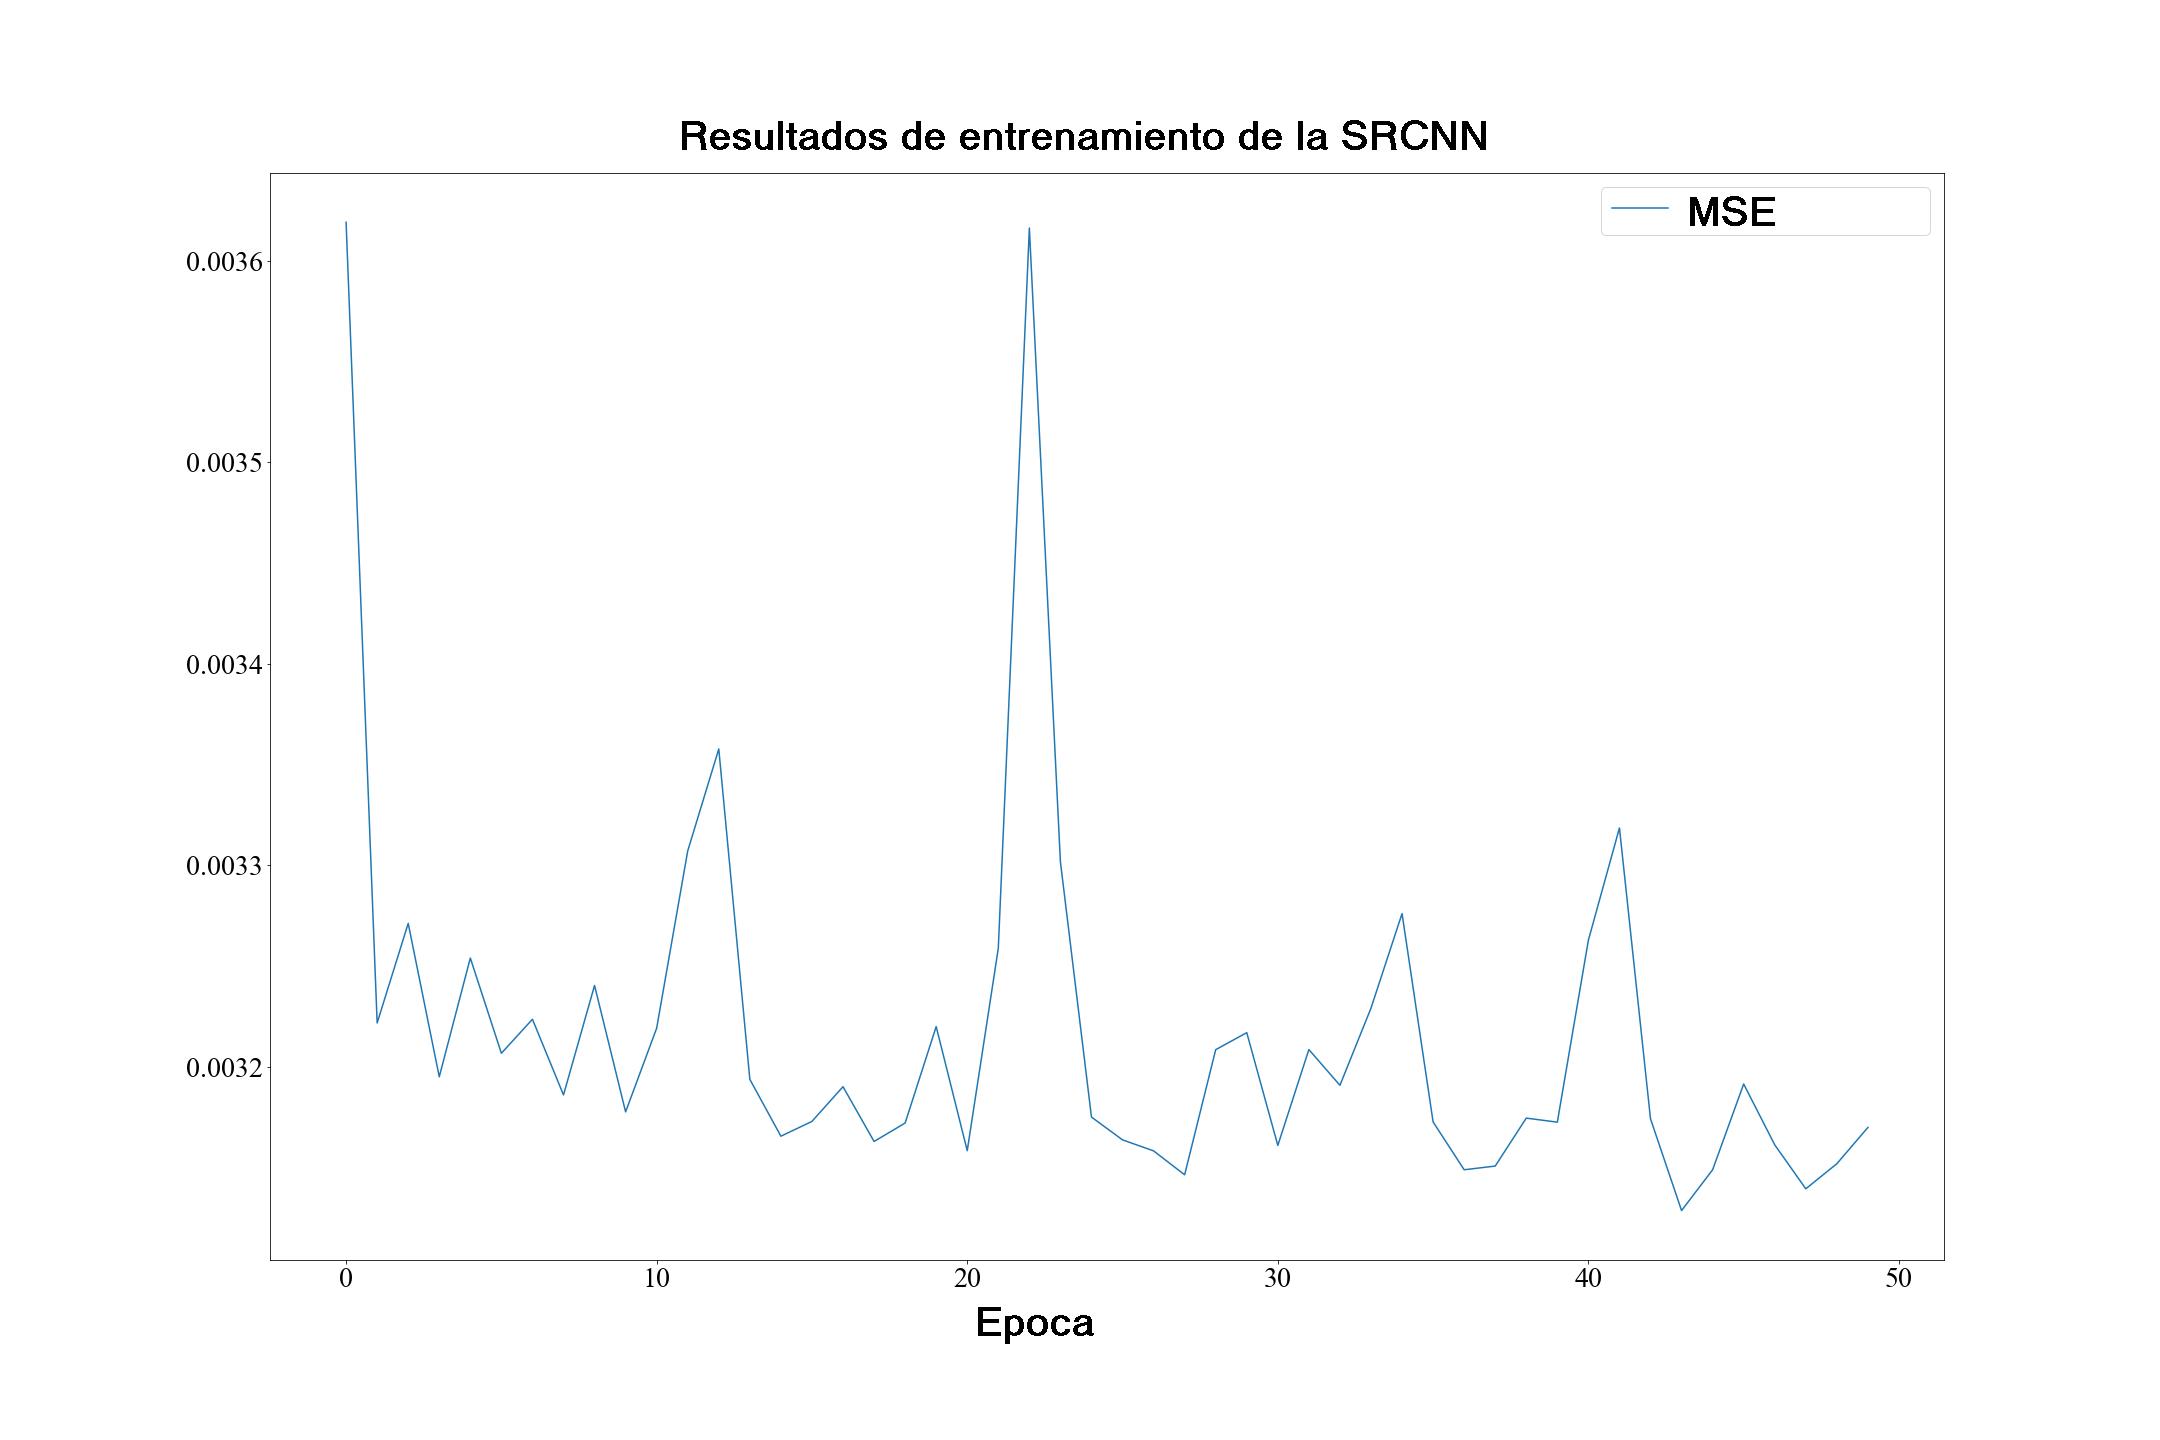
\includegraphics[width=8cm, height=3cm]{TrainingHistory_2475-2525_epochs_4RGB.png}
        \caption{Minimización de función de costo (MSE) de red convolucional $RGB$ con factor de escalamiento $4$}
        \label{fig:SRCNN_MSE_TrainingLoss4RGB}
    \end{figure}
\end{frame}

\begin{frame}{Proceso de entrenamiento modelo $YC_rCb$ y factor $4$ (1/2)}
    \begin{figure}[H]
        \centering
        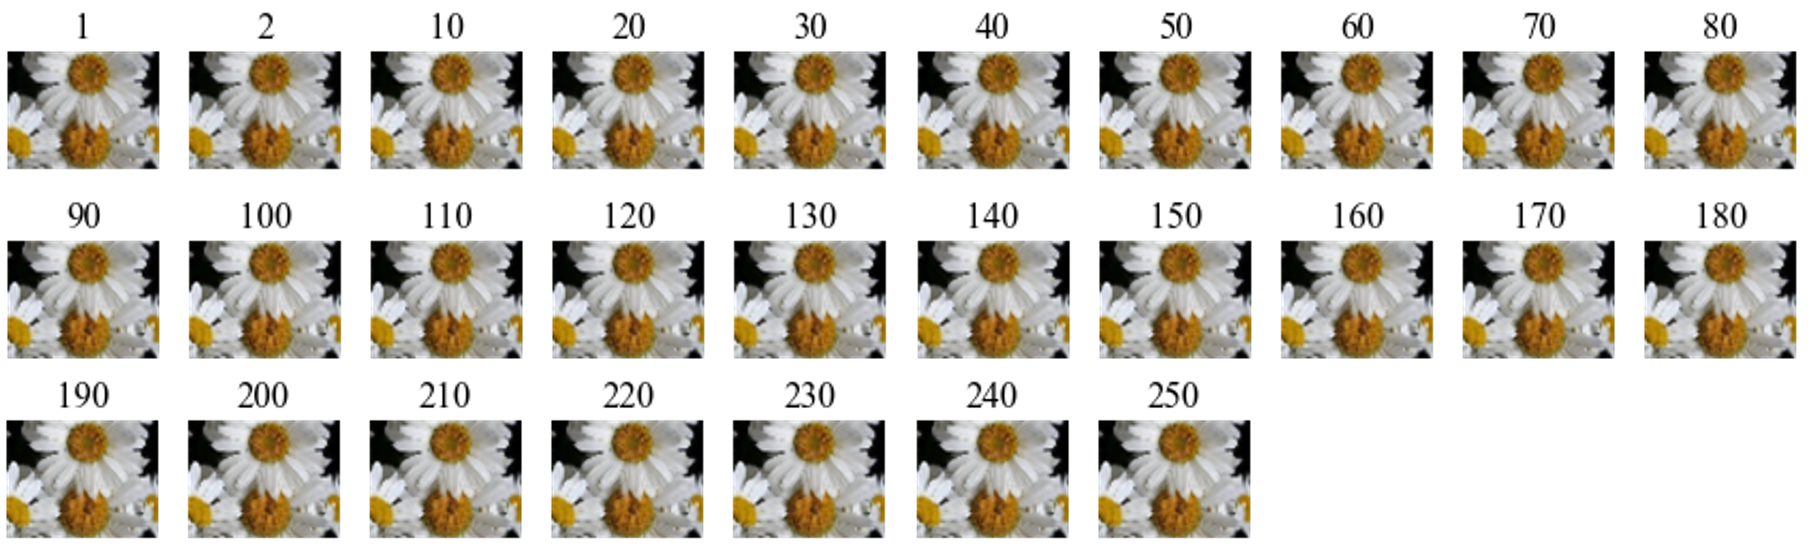
\includegraphics[width=10cm, height=3cm]{ProcesoEntrenamiento_Y4.png}
        \caption{Proceso de aprendizaje de la red convolucional $YC_rC_b$ con factor de escalamiento de $4$}
        \label{fig:SRCNN_MSE_TrainingProcess4Y}
    \end{figure}
\end{frame}
\begin{frame}{Proceso de entrenamiento modelo $YC_rCb$ y factor $4$ (2/2)}
    \begin{figure}[H]
        \centering
        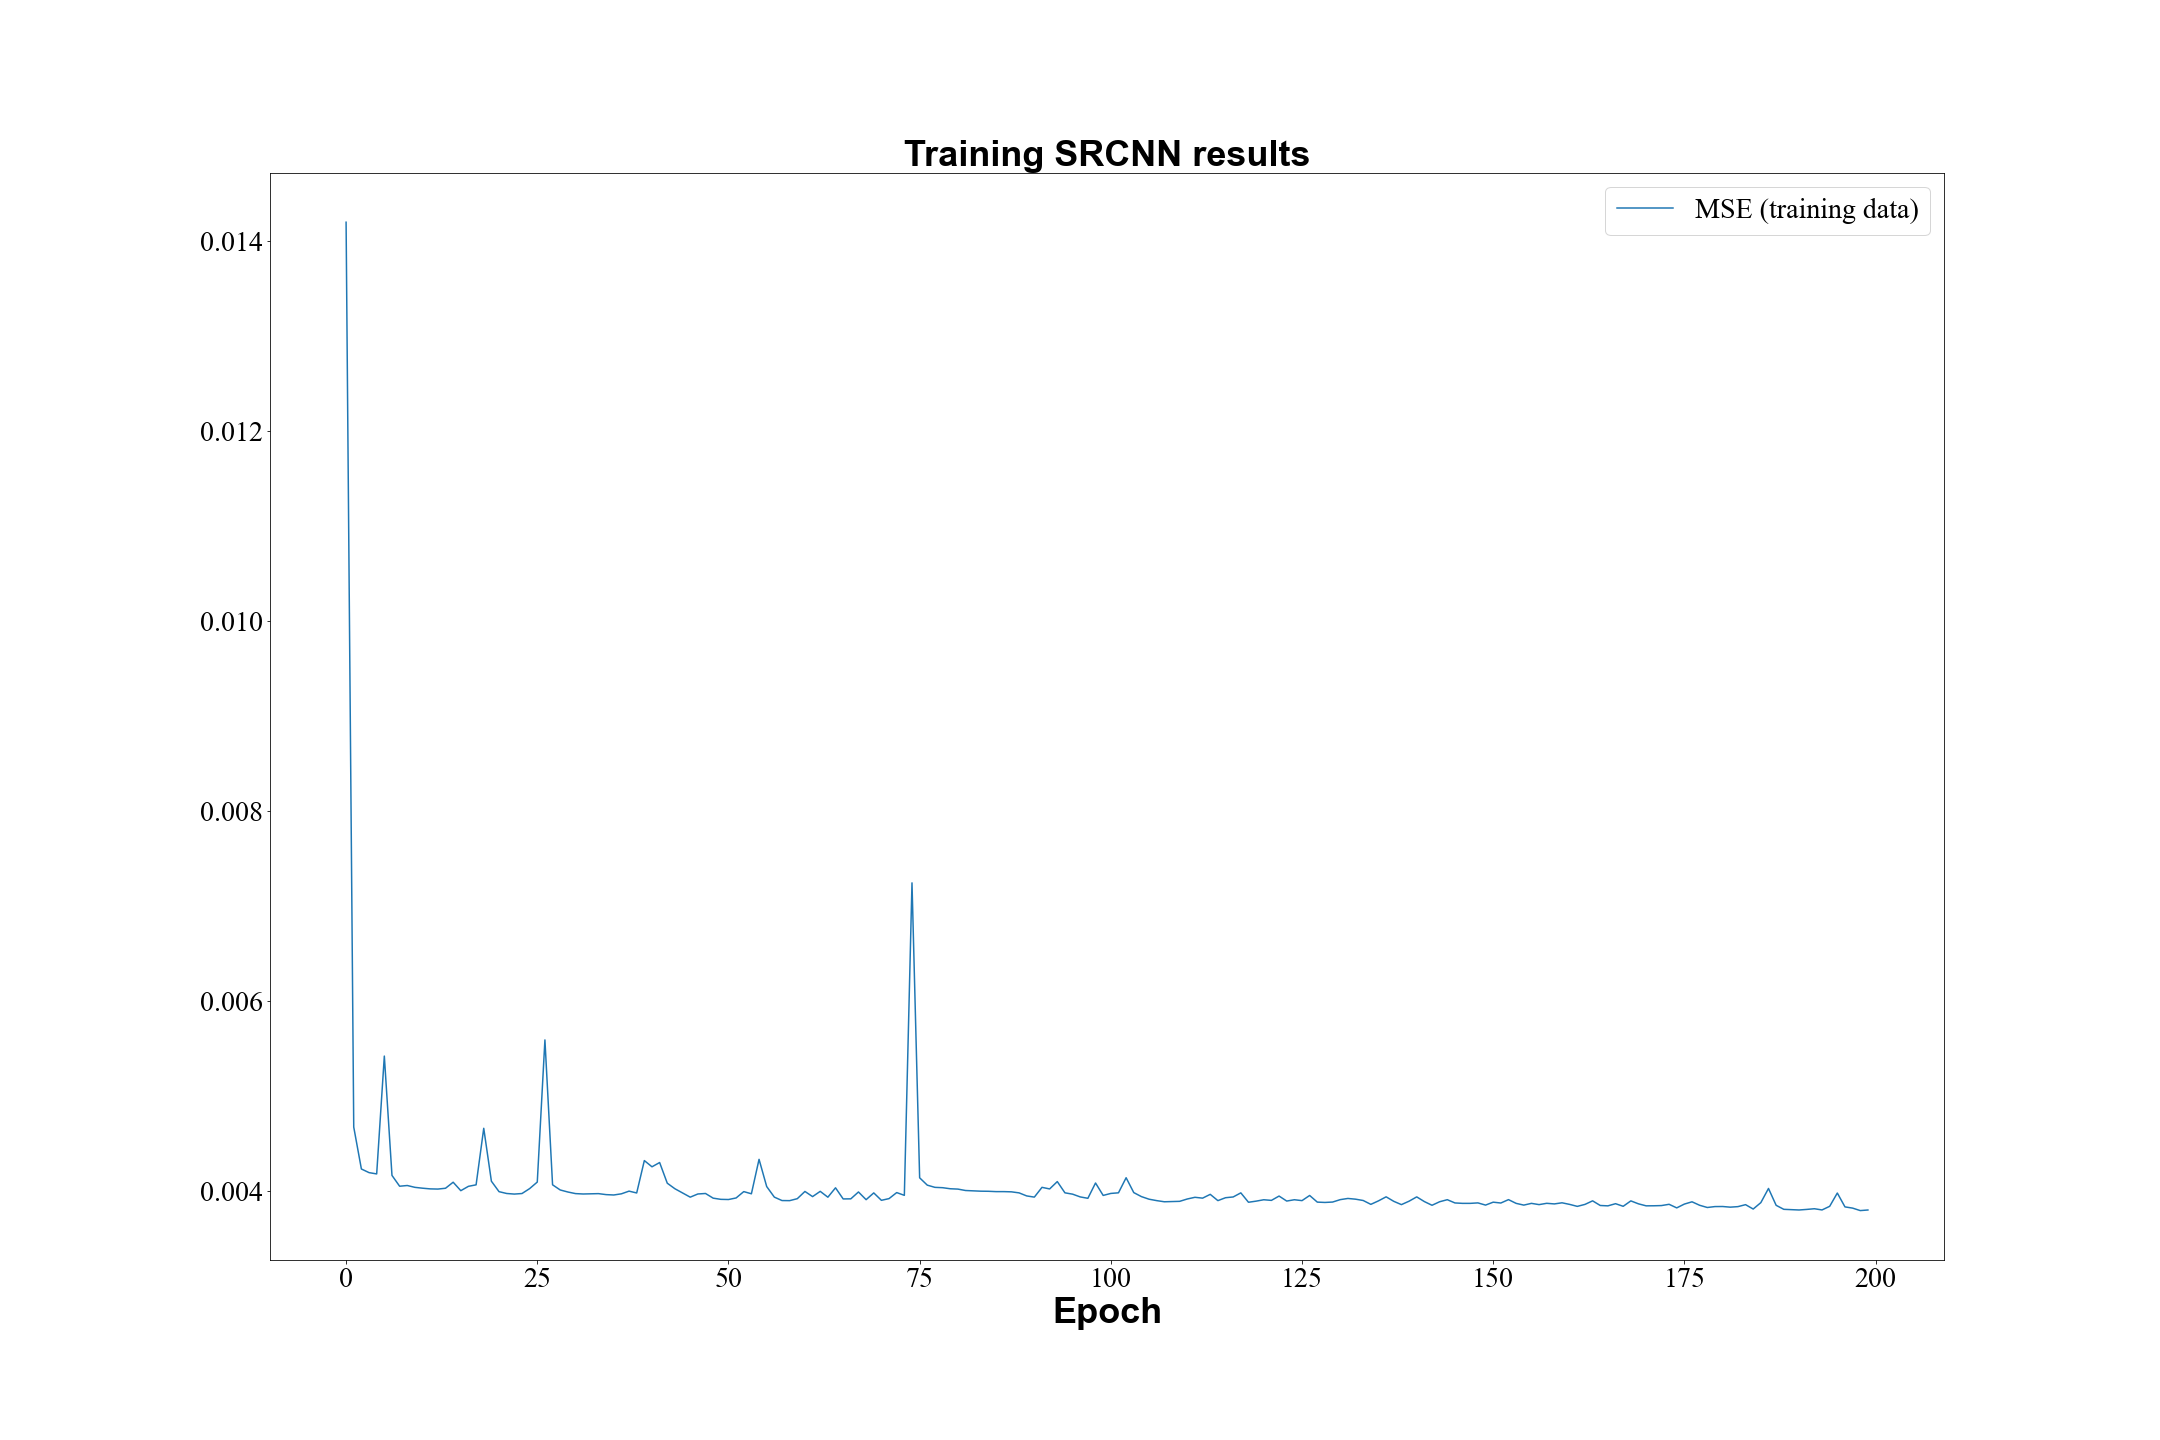
\includegraphics[width=10cm, height=6cm]{TrainingHistory_0-200_epochs_4Y.png}
        \caption{Minimización de función de costo (MSE) de red convolucional $YC_rC_b$ con factor de escalamiento $4$}
        \label{fig:SRCNN_MSE_TrainingLoss4Y}
    \end{figure}
\end{frame}